\documentclass[tikz,border=6pt]{standalone}
\usepackage{tikz}
\usetikzlibrary{arrows.meta}
\definecolor{nebula}{HTML}{6366F1}
\definecolor{spark}{HTML}{14B8A6}
\definecolor{ink}{HTML}{334155}
\begin{document}
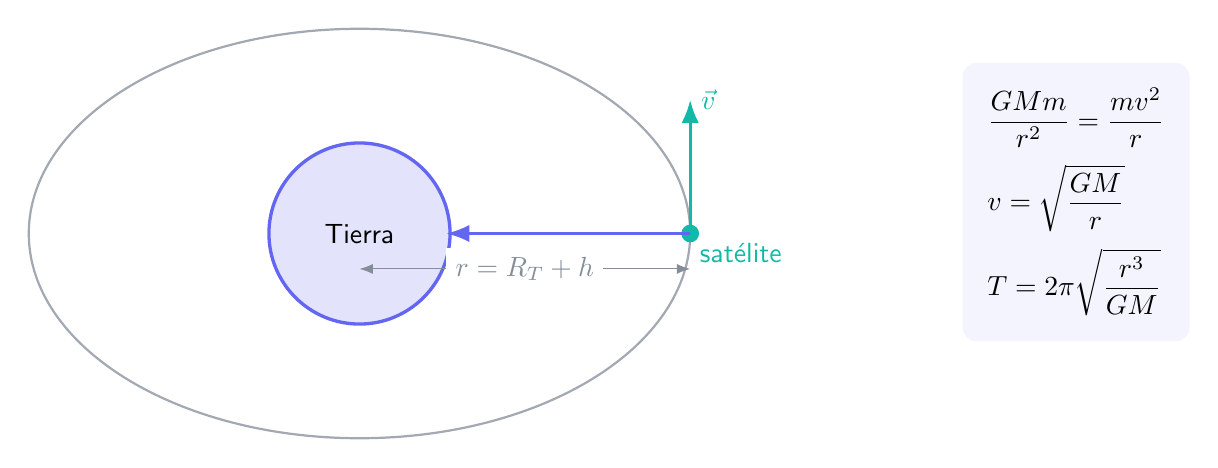
\begin{tikzpicture}[font=\sffamily,>=Latex]
  \draw[thick,ink!45] (0,0) ellipse (4.2 and 2.6);
  \fill[nebula!18] (0,0) circle(1.15);
  \draw[very thick,nebula] (0,0) circle(1.15);
  \node at (0,0) {Tierra};
  \fill[spark] (4.2,0) circle(3.2pt) node[below right] {sat\'elite};
  \draw[->,very thick,spark] (4.2,0)--(4.2,1.7) node[right] {$\vec v$};
  \draw[->,very thick,nebula] (4.2,0)--(1.1,0) node[midway,below=4pt] {$\vec F_g$};
  \draw[<->,thin,ink!60] (0,-0.45)--(4.2,-0.45) node[midway,fill=white] {$r=R_T+h$};
  \node[align=left,fill=nebula!7,rounded corners=5pt,inner sep=9pt] at (9.1,0.4) {$\displaystyle \frac{GMm}{r^2}=\frac{mv^2}{r}$\\[5pt]$\displaystyle v=\sqrt{\frac{GM}{r}}$\\[5pt]$\displaystyle T=2\pi\sqrt{\frac{r^3}{GM}}$};
\end{tikzpicture}
\end{document}
